\documentclass{article}

% If you're new to LaTeX, here's some short tutorials:
% https://www.overleaf.com/learn/latex/Learn_LaTeX_in_30_minutes
% https://en.wikibooks.org/wiki/LaTeX/Basics

% Formatting
\usepackage{tikz}
\usepackage{subfig}
\usepackage{hyperref}
\usepackage{subcaption}
\usepackage[utf8]{inputenc}
\usepackage[margin=1in]{geometry}
\usepackage[titletoc,title]{appendix}

% Math
% https://www.overleaf.com/learn/latex/Mathematical_expressions
% https://en.wikibooks.org/wiki/LaTeX/Mathematics
\usepackage{amsmath,amsfonts,amssymb,mathtools}

% Images
% https://www.overleaf.com/learn/latex/Inserting_Images
% https://en.wikibooks.org/wiki/LaTeX/Floats,_Figures_and_Captions
\usepackage{graphicx,float}

% Tables
% https://www.overleaf.com/learn/latex/Tables
% https://en.wikibooks.org/wiki/LaTeX/Tables

% Algorithms
% https://www.overleaf.com/learn/latex/algorithms
% https://en.wikibooks.org/wiki/LaTeX/Algorithms
\usepackage[ruled,vlined]{algorithm2e}
\usepackage{algorithmic}

% Code syntax highlighting
% https://www.overleaf.com/learn/latex/Code_Highlighting_with_minted
\usepackage{minted}
\usemintedstyle{borland}

% References
% https://www.overleaf.com/learn/latex/Bibliography_management_in_LaTeX
% https://en.wikibooks.org/wiki/LaTeX/Bibliography_Management
\usepackage{biblatex}
\addbibresource{references.bib}

% Title content
\title{
    \textbf{CSE343: Machine Learning} \\ \vspace*{-5pt}
    \textbf{\large{Assignment-3}}
}

\author{\href{mailto:shubham21099@iiitd.ac.in}{Shubham Sharma (2021099)}}
\date{\today}

\geometry{a4paper, left=20mm, right=20mm, top=20mm, bottom=20mm}

\begin{document}

\maketitle

% Abstract
% \begin{abstract}
%     Add your abstract here.
% \end{abstract}

% Introduction and Overview
\section{Section A (Theoretical)}
% Add your introduction and overview here.

% Example Subsection
\subsection*{Solution (a)}
Given
\begin{align*}
\alpha &= 0.01 \quad\\
\text{Inputs: } & [1, 2, 3] \\
\text{Targets: } & [3, 4, 5]
\end{align*}

Assuming initial parameters:
\begin{align*}
w_1 &=  0.5, \quad b_1 = 0.1 \quad \\
w_2 &= -0.3, \quad b_2 = 0.2 \quad \\
\end{align*}

\subsubsection*{Forward Pass}

\textbf{Hidden Layer Activation:} \( h_i = \text{ReLU}(w_1 \cdot x_i + b_1) = max(0, (w_1 \cdot x_i + b_1))\)\\
\textbf{Output Layer Activation:} \( y_i = w_2 \cdot h_i + b_2 \)\\

For \( x = 1 \):
\begin{align*}
    h_1 &= \text{ReLU}(0.5 \cdot 1 + 0.1) = max(0, 0.6) = 0.6 \\
    y_1 &= -0.3 \cdot 0.6 + 0.2 = 0.02
\end{align*}

For \( x = 2 \):
\begin{align*}
    h_2 &= \text{ReLU}(0.5 \cdot 2 + 0.1) = max(0, 1.1) = 1.1 \\
    y_2 &= -0.3 \cdot 1.1 + 0.2 = -0.13
\end{align*}

For \( x = 3 \):
\begin{align*}
    h_3 &= \text{ReLU}(0.5 \cdot 3 + 0.1) = max(0, 1.6) = 1.6 \\
    y_3 &= -0.3 \cdot 1.6 + 0.2 = -0.28
\end{align*}

\subsubsection*{Loss Calculation (Mean Squared Error)}

The MSE loss is calculated as:
\[
\text{Loss} = \frac{1}{3} \sum_{i=1}^{3} (y_i - t_i)^2
\]
where \( t = [3, 4, 5] \).

\[
\text{Loss} = \frac{1}{3} (8.9404 + 17.0149 + 27.8784) = \frac{53.8337}{3} \approx 17.9446
\]

\subsubsection*{Backpropagation: Gradient Computation}
\textbf{Output Layer Gradients (\( w_2 \) and \( b_2 \))}

For each output \( y_i \), we calculate:
\[
\frac{\partial \text{Loss}}{\partial y_i} = \frac{2}{3} (y_i - t_i)
\]

Then, for \( w_2 \):
\[
\frac{\partial \text{Loss}}{\partial w_2} = \frac{1}{3} \sum_{i=1}^{3} \frac{\partial \text{Loss}}{\partial y_i} \cdot h_i
\]

And for \( b_2 \):
\[
\frac{\partial \text{Loss}}{\partial b_2} = \frac{1}{3} \sum_{i=1}^{3} \frac{\partial \text{Loss}}{\partial y_i}
\]


For \( x = 1, y_1 = 0.02, t_1 = 3 \):
\[
\frac{\partial \text{Loss}}{\partial y_1} = \frac{2}{3} (0.02 - 3) = -1.9867
\]

For \( x = 2, y_2 = -0.13, t_2 = 4 \):
\[
\frac{\partial \text{Loss}}{\partial y_2} = \frac{2}{3} (-0.13 - 4) = -2.7533
\]

For \( x = 3, y_3 = -0.28, t_3 = 5 \):
\[
\frac{\partial \text{Loss}}{\partial y_3} = \frac{2}{3} (-0.28 - 5) = -3.52
\]

Gradient for \( w_2 \):
\[
\frac{\partial \text{Loss}}{\partial w_2} = \frac{1}{3} ((-1.9867 \cdot 0.6) + (-2.7533 \cdot 1.1) + (-3.52 \cdot 1.6)) = -3.2842
\]

Gradient for \( b_2 \):
\[
\frac{\partial \text{Loss}}{\partial b_2} = \frac{1}{3} (-1.9867 - 2.7533 - 3.52) = -2.7533
\]

\vspace{10pt}
\hspace{-20pt}
\textbf{Hidden Layer Gradients (\( w_1 \) and \( b_1 \))}

Gradient of Loss w.r.t \( h_i \):
\[
\frac{\partial \text{Loss}}{\partial h_i} = \frac{\partial \text{Loss}}{\partial y_i} \cdot w_2
\]

Gradient of Loss w.r.t \( w_1 \) and \( b_1 \):
\[
\frac{\partial \text{Loss}}{\partial w_1} = \frac{1}{3} \sum_{i=1}^{3} \frac{\partial \text{Loss}}{\partial h_i} \cdot x_i \cdot \text{ReLU}'(z_i)
\]
\[
\frac{\partial \text{Loss}}{\partial b_1} = \frac{1}{3} \sum_{i=1}^{3} \frac{\partial \text{Loss}}{\partial h_i} \cdot \text{ReLU}'(z_i)
\]
where \( \text{ReLU}'(z_i) \) is the derivative of ReLU at \( z_i = w_1 \cdot x_i + b_1 \).

\vspace{5pt}
For \( x = 1, \text{ReLU}'(0.6) = 1 \):
\[
\frac{\partial \text{Loss}}{\partial h_1} = -1.9867 \cdot (-0.3) = 0.59601
\]

For \( x = 2 \), \( \text{ReLU}'(1.1) = 1 \):

\[
\frac{\partial \text{Loss}}{\partial h_2} = -2.7533 \cdot (-0.3) = 0.826
\]

For \( x = 3 \), \( \text{ReLU}'(1.6) = 1 \):

\[
\frac{\partial \text{Loss}}{\partial h_3} = -3.52 \cdot (-0.3) = 1.056
\]

Gradient for \( w_1 \):

\[
\frac{\partial \text{Loss}}{\partial w_1} = \frac{1}{3} (0.59601 \cdot 1 + 0.826 \cdot 2 + 1.056 \cdot 3)
\]
\[
= \frac{1}{3} (0.59601 + 1.652 + 3.168) = \frac{5.41601}{3} \approx 1.8053
\]

Gradient for \( b_1 \):

\[
\frac{\partial \text{Loss}}{\partial b_1} = \frac{1}{3} (0.59601 + 0.826 + 1.056) = \frac{2.47801}{3} \approx 0.826
\]

\subsubsection*{Parameter Update}

Using a given learning rate \( \alpha = 0.01 \):
\vspace{5pt}

Update \( w_2 \):

\[
w_2 = w_2 - \alpha \cdot \frac{\partial \text{Loss}}{\partial w_2} = -0.3 - 0.01 \cdot (-3.2842) = -0.3 + 0.032842 = \textbf{-0.2672}
\]

Update \( b_2 \):

\[
b_2 = b_2 - \alpha \cdot \frac{\partial \text{Loss}}{\partial b_2} = 0.2 - 0.01 \cdot (-2.7533) = 0.2 + 0.0275 = \textbf{0.2275}
\]

Update \( w_1 \):

\[
w_1 = w_1 - \alpha \cdot \frac{\partial \text{Loss}}{\partial w_1} = 0.5 - 0.01 \cdot 1.8053 = 0.5 - 0.01805 = \textbf{0.4819}
\]

Update \( b_1 \):

\[
b_1 = b_1 - \alpha \cdot \frac{\partial \text{Loss}}{\partial b_1} = 0.1 - 0.01 \cdot 0.826 = 0.1 - 0.00826 = \textbf{0.0917}
\]

\subsubsection*{Updated Parameters}


\[
w_1 = 0.4819
\]
\[
b_1 = 0.0917
\]
\[
w_2 = -0.2672
\]
\[
b_2 = 0.2275
\]


\vspace{10pt}
\subsection*{Solution (b)}
\begin{table}[H]
    \centering
    \begin{tabular}{|c|c|c|c|}
        \hline
        \textbf{Class} & \textbf{x}_1 & \textbf{x}_2 & \textbf{Label} \\ \hline
        + & 0 & 0 & + \\ \hline
        + & 1 & 0 & + \\ \hline
        + & 0 & 1 & + \\ \hline
        - & 1 & 1 & - \\ \hline
        - & 2 & 2 & - \\ \hline
        - & 2 & 0 & - \\ \hline
    \end{tabular}
    \caption{Given Datapoints}
\end{table}
\subsubsection*{a) Linear Separability of Points}
\begin{center}
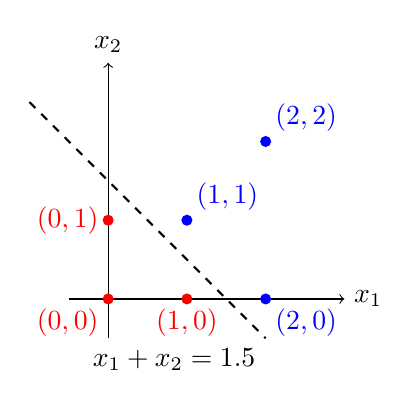
\begin{tikzpicture}[scale=1]
    \draw[->] (-0.5, 0) -- (3, 0) node[right] {$x_1$};
    \draw[->] (0, -0.5) -- (0, 3) node[above] {$x_2$};

    \fill[red] (0, 0) circle (2pt) node[below left] {$(0,0)$};
    \fill[red] (1, 0) circle (2pt) node[below] {$(1,0)$};
    \fill[red] (0, 1) circle (2pt) node[left] {$(0,1)$};

    \fill[blue] (1, 1) circle (2pt) node[above right] {$(1,1)$};
    \fill[blue] (2, 2) circle (2pt) node[above right] {$(2,2)$};
    \fill[blue] (2, 0) circle (2pt) node[below right] {$(2,0)$};

    \draw[thick, dashed] (-1.0, 2.5) -- (2.0, -0.5) node[below left] {$x_1 + x_2 = 1.5$};

\end{tikzpicture}
\end{center}

\begin{center}
\begin{tabular}{|c|c|c|c|}
    \hline
    \textbf{Class} & \textbf{x}_1 & \textbf{x}_2 & $\textbf{x}_1 + \textbf{x}_2$ \\
    \hline
    $+$ & 0 & 0 & 0 \\ \hline
    $+$ & 1 & 0 & 1 \\ \hline
    $+$ & 0 & 1 & 1 \\ \hline
    $-$ & 1 & 1 & 2 \\ \hline
    $-$ & 2 & 2 & 4 \\ \hline
    $-$ & 2 & 0 & 2 \\ \hline
\end{tabular}
\end{center}

From the table:
\begin{itemize}
    \item For the positive class, $x_1 + x_2$ values are 0 and 1.
    \item For the negative class, $x_1 + x_2$ values are 2 and 4.
\end{itemize}

We choose the line $x_1 + x_2 = 1.5$ as the separating line:
\begin{itemize}
    \item All positive points satisfy $x_1 + x_2 \leq 1.5$.
    \item All negative points satisfy $x_1 + x_2 > 1.5$.
\end{itemize}

\vspace{5pt}
Thus, the points are \textbf{linearly separable} by the line $x_1 + x_2 = 1.5$. Also, from the graph, it is clearly visible that data points are \textbf{linearly separable}.


\subsubsection*{b) Finding Weight Vector and Support Vector}

From the Graph, I observed the below support vectors:
\begin{itemize}
    \item Positive support vectors: $(0, 1)$ and $(1, 0)$
    \item Negative support vectors: $(1, 1)$ and $(2, 0)$
\end{itemize}

Using support vectors:
\begin{align}
    w_1 \cdot 0 + w_2 \cdot 1 + b &= 1, \\
    w_1 \cdot 1 + w_2 \cdot 0 + b &= 1, \\
    w_1 \cdot 1 + w_2 \cdot 1 + b &= -1, \\
    w_1 \cdot 2 + w_2 \cdot 0 + b &= -1.
\end{align}

Solving these equations step-by-step:
\begin{enumerate}
    \item From the equation (1), we have $w_2 = 1 - b$.
    \item Substitute $w_2 = 1 - b$ into the equation (3):
    \begin{align*}
        w_1 + (1 - b) + b &= -1 \\
        w_1 + 1 &= -1 \\
        w_1 &= -2.
    \end{align*}
    \item Substitute $w_1 = -2$ into the equation (2):
    \begin{align*}
        -2 + b &= 1 \\
        b &= 3.
    \end{align*}
    \item Substitute $b = 3$ into the equation (1) to find $w_2$:
    \begin{align*}
        w_2 &= 1 - 3 \\
        w_2 &= -2.
    \end{align*}
\end{enumerate}

So,
\[
\textbf{w}_1 \textbf{=} \textbf{-2}, \quad \textbf{w}_2 \textbf{= -2}, \quad \textbf{b = 3}
\]

The equation of the maximum margin hyperplane is:
\[
-2x_1 - 2x_2 + 3 = 0,
\]
or equivalently:
\[
x_1 + x_2 = 1.5.
\]

\vspace{10pt}
\subsection*{Solution (c)}
\subsubsection*{(a) Calculate the margin of the classifier.}

Margin \( \gamma \) for an SVM is:
\[
\gamma = \frac{2}{\sqrt{w_1^2 + w_2^2}}
\]

\hspace{-18pt}
Substitute \( w_1 = -2 \) and \( w_2 = 0 \):
\[
\sqrt{w_1^2 + w_2^2} = \sqrt{(-2)^2 + 0^2} = \sqrt{4} = 2
\]
Thus, the margin is:
\[
\gamma = \frac{2}{2} = \textbf{1}
\]

\subsubsection*{(b) Identify the support vectors.}

Support vectors are the points that lie on the margin boundaries, where \( \textbf{y (w} \cdot \textbf{x + b) = 1} \).

\[
\begin{array}{|c|c|c|c|c|c|}
\hline
\textbf{Sample No.} & \textbf{x}_1 & \textbf{x}_2 & \textbf{y} & \textbf{w} \cdot \textbf{x} + \textbf{b} & \textbf{y} (\textbf{w} \cdot \textbf{x} + \textbf{b}) \\
\hline
1 & 1 & 2 & +1 & (-2 \cdot 1) + (0 \cdot 2) + 5 = 3 & 1 \cdot 3 = 3 \\
2 & 2 & 3 & +1 & (-2 \cdot 2) + (0 \cdot 3) + 5 = 1 & 1 \cdot 1 = \textbf{1} \\
3 & 3 & 3 & -1 & (-2 \cdot 3) + (0 \cdot 3) + 5 = -1 & -1 \cdot -1 = \textbf{1} \\
4 & 4 & 1 & -1 & (-2 \cdot 4) + (0 \cdot 1) + 5 = -3 & -1 \cdot -3 = 3 \\
\hline
\end{array}
\]

From the table, we observe that \textbf{Samples 2 and 3} satisfy \( y (w \cdot x + b) = 1 \), so they are the support vectors.


\subsubsection*{(c) Predict the class of a new point}
Using the decision function:
\[
f(x) = w \cdot x + b = -2 \cdot x_1 + 0 \cdot x_2 + 5
\]
For \( (x_1, x_2) = (1, 3) \):
\[
f(x) = -2 \cdot 1 + 0 \cdot 3 + 5 = -2 + 5 = 3
\]
Since \( f(x) > 0 \), the classifier predicts \( \textbf{y = +1} \) for this new point.


\vspace{10pt} % add 10pt of vertical space
\section{Section C (Algorithm implementation using packages)}
\subsection*{Part 1: Normalization and Visualization of Sample Images}
\subsubsection*{a) Visualization of Sample Images}
\begin{figure}[H] % h = here, t = top, b = bottom, etc.
    \centering
    \begin{minipage}{1\linewidth}
        \centering
        \includegraphics[scale=0.4]{assets/sample_images.png}
        \caption{First 10 Sample Images from Test Dataset}{}
        \label{fig:1c}
    \end{minipage}
\end{figure}

All the data points in the dataset are first normalized by dividing them by 255.0 then the first 10 images from the test dataset are displayed after reshaping the features to 28x28.

\subsection*{Part 2: Training model and Calculating Training and Validation Loss}
\begin{figure}[H] % h = here, t = top, b = bottom, etc.
    \centering
    \begin{minipage}{0.49\linewidth}
        \centering
        \includegraphics[width=\linewidth]{assets/2-logistic.png}
        \caption{Losses vs Epochs for \textbf{Logistic} Activation}{}
        \label{fig:b-1}
    \end{minipage}
    \hfill
    \begin{minipage}{0.49\linewidth}
        \centering
        \includegraphics[width=\linewidth]{assets/2-tanh.png}
        \caption{Losses vs Epochs for \textbf{Tanh} Activation}{}
        \label{fig:b-2}
    \end{minipage}
\end{figure}

\begin{figure}[H] % h = here, t = top, b = bottom, etc.
    \centering
    \begin{minipage}{0.49\linewidth}
        \centering
        \includegraphics[width=\linewidth]{assets/2-relu.png}
        \caption{Losses vs Epochs for \textbf{ReLU} Activation}{}
        \label{fig:b-1}
    \end{minipage}
    \hfill
    \begin{minipage}{0.49\linewidth}
        \centering
        \includegraphics[width=\linewidth]{assets/2-identity.png}
        \caption{Losses vs Epochs for \textbf{Identity} Activation}{}
        \label{fig:b-2}
    \end{minipage}
\end{figure}

\begin{table}[H]
    \centering
    \begin{tabular}{|c|c|}
        \hline
        \textbf{Activation Function} & \textbf{Test Accuracy}\\ \hline
        Logistic & 0.533\\ \hline
        Tanh & 0.8375\\ \hline
        ReLU & 0.835\\ \hline
        Identity & 0.831\\ \hline
    \end{tabular}
    \caption{Different Activation Functions and their Accuracies}
\end{table}

\hspace{0pt}Best performing Activation function is \textbf{tanh} and some major observations are below:-

\begin{enumerate}
\item Logistic activation has poor performance (53.3\%) due to vanishing gradients, which hinders the learning of complex patterns.
\item Other activation functions reduce vanishing gradients—Tanh scales to (-1,1), ReLU introduces sparsity, and Identity allows linear propagation, leading to better performance around 83\%.
\item Random Variability in weight initialization causes slight differences in convergence paths, affecting accuracy.
\item I observed on each run Tanh, ReLU, or Identity to perform best depending on the random factors such as random weights, convergence path and different local minima etc.
\end{enumerate}

\subsection*{Part 3: Grid Search CV using Best Activation Function}
\begin{table}[H]
    \centering
    \begin{tabular}{|c|c|c|} % Adjust column widths as needed
        \hline
        \textbf{Hyperparameter} & \textbf{Values (Grid Search)} & \textbf{Best Value} \\
        \hline
        solver & \{'adam', 'sgd'\} & 'adam'\\ \hline
        learning\_rate\_init & \{0.1, 0.0001, 2e-3, 2e-4, 2e-5\} & 2e-3 \\ \hline
        batch\_size & \{64, 128, 256\} & 128 \\ \hline
    \end{tabular}
    \caption{MLP Classifier Hyperparameter Grid and Best Parameters from Grid Search}
\end{table}

\hspace{-3pt}
Performed the Grid Search CV with 3 folds. I performed Gird Search on three parameters, such as solver, learning\_rate and batch\_size, which resulted in a total of \textbf{30 combinations} and \textbf{90 fits}. In all of the combinations, the activation function we used is the best activation function that we found in the previous part.

\subsection*{Part 4: Training MLP Regressor Model for Image Regeneration Task}
\subsubsection*{a) Layer Sizes}
\begin{table}[H]
    \centering
    \begin{tabular}{|c|c|} % Adjust column widths as needed
        \hline
        \textbf{Layer Size} & \textbf{[128, 64, 32, 64, 128]} \\ \hline
    \end{tabular}
    % \caption{MLP Classifier Hyperparameter Grid and Best Parameters from Grid Search}
\end{table}

\hspace{-3pt}
Chosen layer sizes \textbf{c = 128}, \textbf{b = 64}, and \textbf{a = 32} are ideal for regeneration tasks as they form symmetric structures and compress and reconstruct images efficiently.

\subsubsection*{b) Plotting Curves}
\begin{figure}[H] % h = here, t = top, b = bottom, etc.
    \centering
    \begin{minipage}{0.49\linewidth}
        \centering
        \includegraphics[width=\linewidth]{assets/4-relu.png}
        \caption{Losses vs Epochs for \textbf{ReLU} Activation}{}
        \label{fig:b-1}
    \end{minipage}
    \hfill
    \begin{minipage}{0.49\linewidth}
        \centering
        \includegraphics[width=\linewidth]{assets/4-identity.png}
        \caption{Losses vs Epochs for \textbf{identity} Activation}{}
        \label{fig:b-2}
    \end{minipage}
\end{figure}

As clearly visible from both graphs, the loss continuously decreases with each epoch, and we conclude that our models are learning correctly.

\subsubsection*{c) Training Models}
\begin{table}[H]
    \centering
    \begin{tabular}{|c|c|}
        \hline
        \textbf{Activation Function} & \textbf{RMSE Score}\\ \hline
        ReLU & 0.145426\\ \hline
        Identity & 0.154098\\ \hline
    \end{tabular}
    \caption{Different Activation Functions and their RMSE Score}
\end{table}

\subsubsection*{d) Visualization of Regenerated Images}
\begin{figure}[H] % h = here, t = top, b = bottom, etc.
    \centering
    \begin{minipage}{1\linewidth}
        \centering
        \includegraphics[scale=0.4]{assets/comparision.png}
        \caption{Comparision of First 10 Sample Images from Test Dataset}{}
        \label{fig:1c}
    \end{minipage}
\end{figure}

\hspace{0pt}\textbf{Observations:-}

\begin{enumerate}
\item I observed that the model which uses the ReLU activation function produces slightly clearer and sharper regenerated images compared to the Identity activation function because ReLU is a non-linear activation function and better captures complex patterns.
\item Images generated using the Identity activation function are slightly blurred compared to ReLU, which directly shows that the Identity activation function is not good at capturing complex details.
\item In Images generated by the ReLU activation function, the object outlines are slightly sharper than the identity, which makes it visually easy to recognize the object in the image.
\end{enumerate}

\subsection*{Part 5: Extracting Features and Training Classifiers on Extracted Features}
\begin{figure}[H] % h = here, t = top, b = bottom, etc.
    \centering
    \begin{minipage}{0.49\linewidth}
        \centering
        \includegraphics[width=\linewidth]{assets/5-relu.png}
        \caption{Losses vs Epochs for \textbf{ReLU} Activation}{}
        \label{fig:b-1}
    \end{minipage}
    \hfill
    \begin{minipage}{0.49\linewidth}
        \centering
        \includegraphics[width=\linewidth]{assets/5-identity.png}
        \caption{Losses vs Epochs for \textbf{identity} Activation}{}
        \label{fig:b-2}
    \end{minipage}
\end{figure}

\begin{table}[H]
    \centering
    \begin{tabular}{|c|c|}
        \hline
        \textbf{Activation Function} & \textbf{Test Accuracy}\\ \hline
        ReLU & 0.692\\ \hline
        Identity & 0.741\\ \hline
    \end{tabular}
    \caption{Different Activation Functions and their Accuracies}
\end{table}

\textbf{Contrast of Part 5 with Part 2 is below:-}
\begin{enumerate}
\item In Part 2, the classifier model with ReLU and Identity activation gives 83.5\% and 83.1\% accuracy, respectively, while in Part 5, the classifier model with ReLU and Identity activation gives 69.2\% and 74.1\% accuracy, respectively.
\end{enumerate}

\hspace{-20pt}
\textbf{Possible Reason:-}
\begin{enumerate}
\item Extracted feature vectors keep the important pattern and make them ideal for quickly training smaller classifiers.
\item Feature vectors reduce data complexity but keep essential details, helping smaller classifiers in achieving decent accuracy.
\item Features from deeper layers capture detailed patterns and boost image classification accuracy.
\end{enumerate}
% \clearpage % This ensures the page break happens here

% \vspace{10pt}
% \subsection*{Solution (f)}
% \subsubsection*{Early Stopping and its Effect of Overfitting and Generalization}
% \begin{figure}[H] % h = here, t = top, b = bottom, etc.
%     \centering
%     \begin{minipage}{0.49\linewidth}
%         \centering
%         \includegraphics[width=\linewidth]{assets/fV.png}
%         \caption{Validation Dataset}{}
%         \label{fig:b-1}
%     \end{minipage}
%     \hfill
%     \begin{minipage}{0.49\linewidth}
%         \centering
%         \includegraphics[width=\linewidth]{assets/fT.png}
%         \caption{Test Dataset}{}
%         \label{fig:b-2}
%     \end{minipage}
%     \caption*{Comparing impact of Early Stopping \& No Early Stopping}
% \end{figure}

% \hspace{-20pt}
% \begin{table}[H]
% \centering
% \resizebox{\textwidth}{!}{
% \begin{tabular}{|c|c|c|c|c|c|c|}
% \hline
% $\alpha$ & Regularization & $\lambda$ & Accuracy (ES/NO-ES) & Precision (ES/NO-ES) & Recall (ES/NO-ES) & F1 (ES/NO-ES) \\ 
% \hline
% 1     & L1  & 0.001  & (0.8415, 0.8415) & (0.3636, 0.3636) & (0.0476, 0.0476) & (0.0842, 0.0842) \\ \hline
% 0.1   & L1  & 0.001  & (0.8525, 0.8488) & (0.6364, 0.5714) & (0.0833, 0.0476) & (0.1474, 0.0879) \\ \hline
% 0.01  & L1  & 0.001  & (0.8543, 0.8415) & (0.5833, 0.4286) & (0.1667, 0.1071) & (0.2593, 0.1714) \\ \hline
% 0.001 & L1  & 0.001  & (0.8397, 0.8415) & (0.3333, 0.3636) & (0.0476, 0.0476) & (0.0833, 0.0842) \\ \hline
% 1     & L2  & 1e-05  & (0.8415, 0.8415) & (0.3636, 0.3636) & (0.0476, 0.0476) & (0.0842, 0.0842) \\ \hline
% 0.1   & L2  & 1e-05  & (0.8525, 0.8488) & (0.6364, 0.5714) & (0.0833, 0.0476) & (0.1474, 0.0879) \\ \hline
% 0.01  & L2  & 1e-05  & (0.8543, 0.8415) & (0.5833, 0.4286) & (0.1667, 0.1071) & (0.2593, 0.1714) \\ \hline
% 0.001 & L2  & 1e-05  & (0.8397, 0.8397) & (0.3333, 0.3333) & (0.0476, 0.0476) & (0.0833, 0.0833) \\ 
% \hline
% \end{tabular}
% }
% \caption{Comparison of Early Stopping (ES) and No Early Stopping (NO-ES).}
% \end{table}



% \hspace{-15pt}To prevent overfitting, I choose the early stopping parameter as patience = 10 and min\_delta = 1e-3. This means that training will stop if the validation loss does not improve by at least 1e-3 for 10 consecutive epochs.
% \vspace{5pt}
% \newline\hspace{-15pt}After trying eight different combinations of learning rate ($\alpha$) = \{1, 0.1, 0.01, 0.001\} and L1, L2 regularization, I come to the conclusion that early stopping stops the overfitting and promotes the generalization of the unseen test data. As it will be clearly visible in the metrics data. From all combinations of models in which early stopping is enabled, has better accuracy, precision, recall, and F1-score.

\end{document}
